\newpage


\section{Grundlagen}

\subsection{Laravel}

\subsection{Laravel Nova}
Um Entwickler dabei zu unterstützen, besonders effizient und einfach, Administrationsinterfaces für Laravel Anwendungen zu entwickeln, wurde ein kostenpflichtiges first-party Framework entwickelt und veröffentlicht.\cite{laravel-nova}
Oftmals haben Laravel Anwendungen eine öffentliche Website, einen Administrationsbereich für die Verwaltung der Daten und eine Programmierschnittstelle (API).\cite{laravel-up-and-running}
Mit Laravel selbst lässt sich sehr gut eine API abdecken, ebenso ist es für öffentliche Websites designt.
Laravel Nova setzt also genau in dem Bereich an, den Entwickler in der Regel individuell aufbauen.

\subsection{Methoden}
\begin{figure}[h!]
    \centering
    \caption{Themenfeldanalyse (Beispiel einer Grafik im Hauptteil)}
    \label{fig:themenfeldanalyse}
    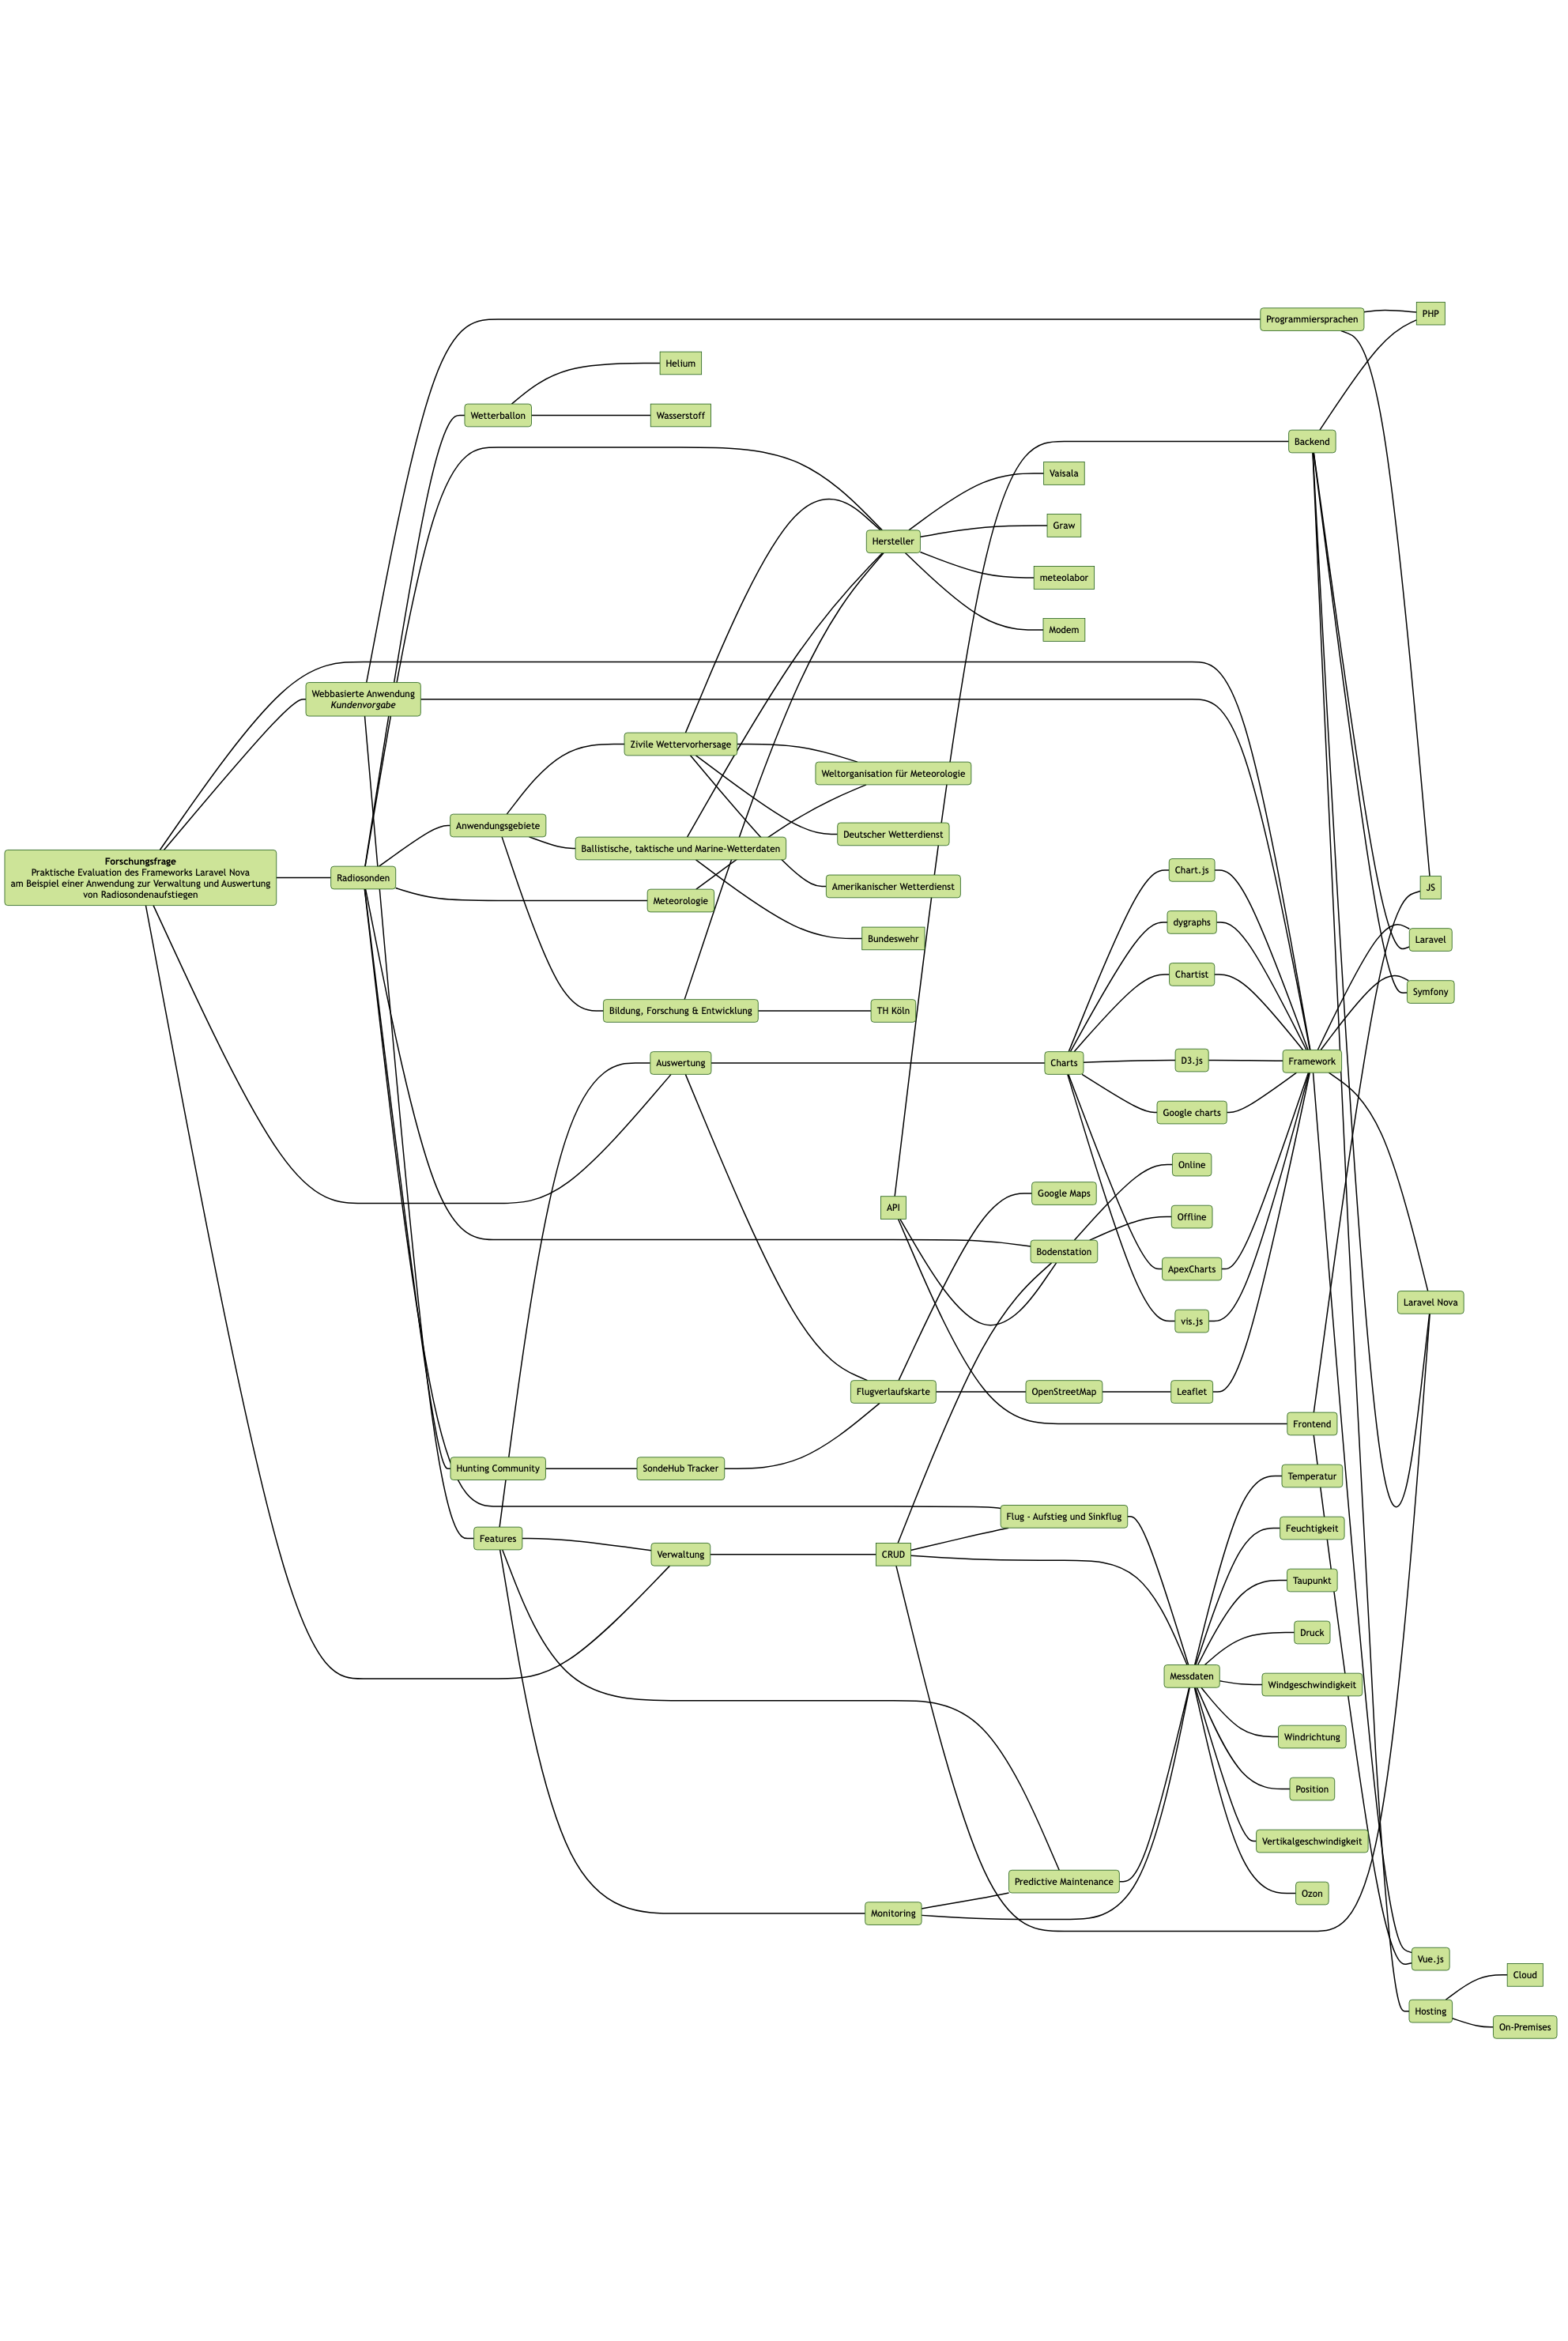
\includegraphics[scale=0.23]{images/themenfeldanalyse}
\end{figure}
